\section{Resultados}
\begin{frame}
	\frametitle{Control mediante Arduino Mega 2560}
	\begin{columns}
		\begin{column}{0.5\linewidth}
			\begin{figure}
				\centering
				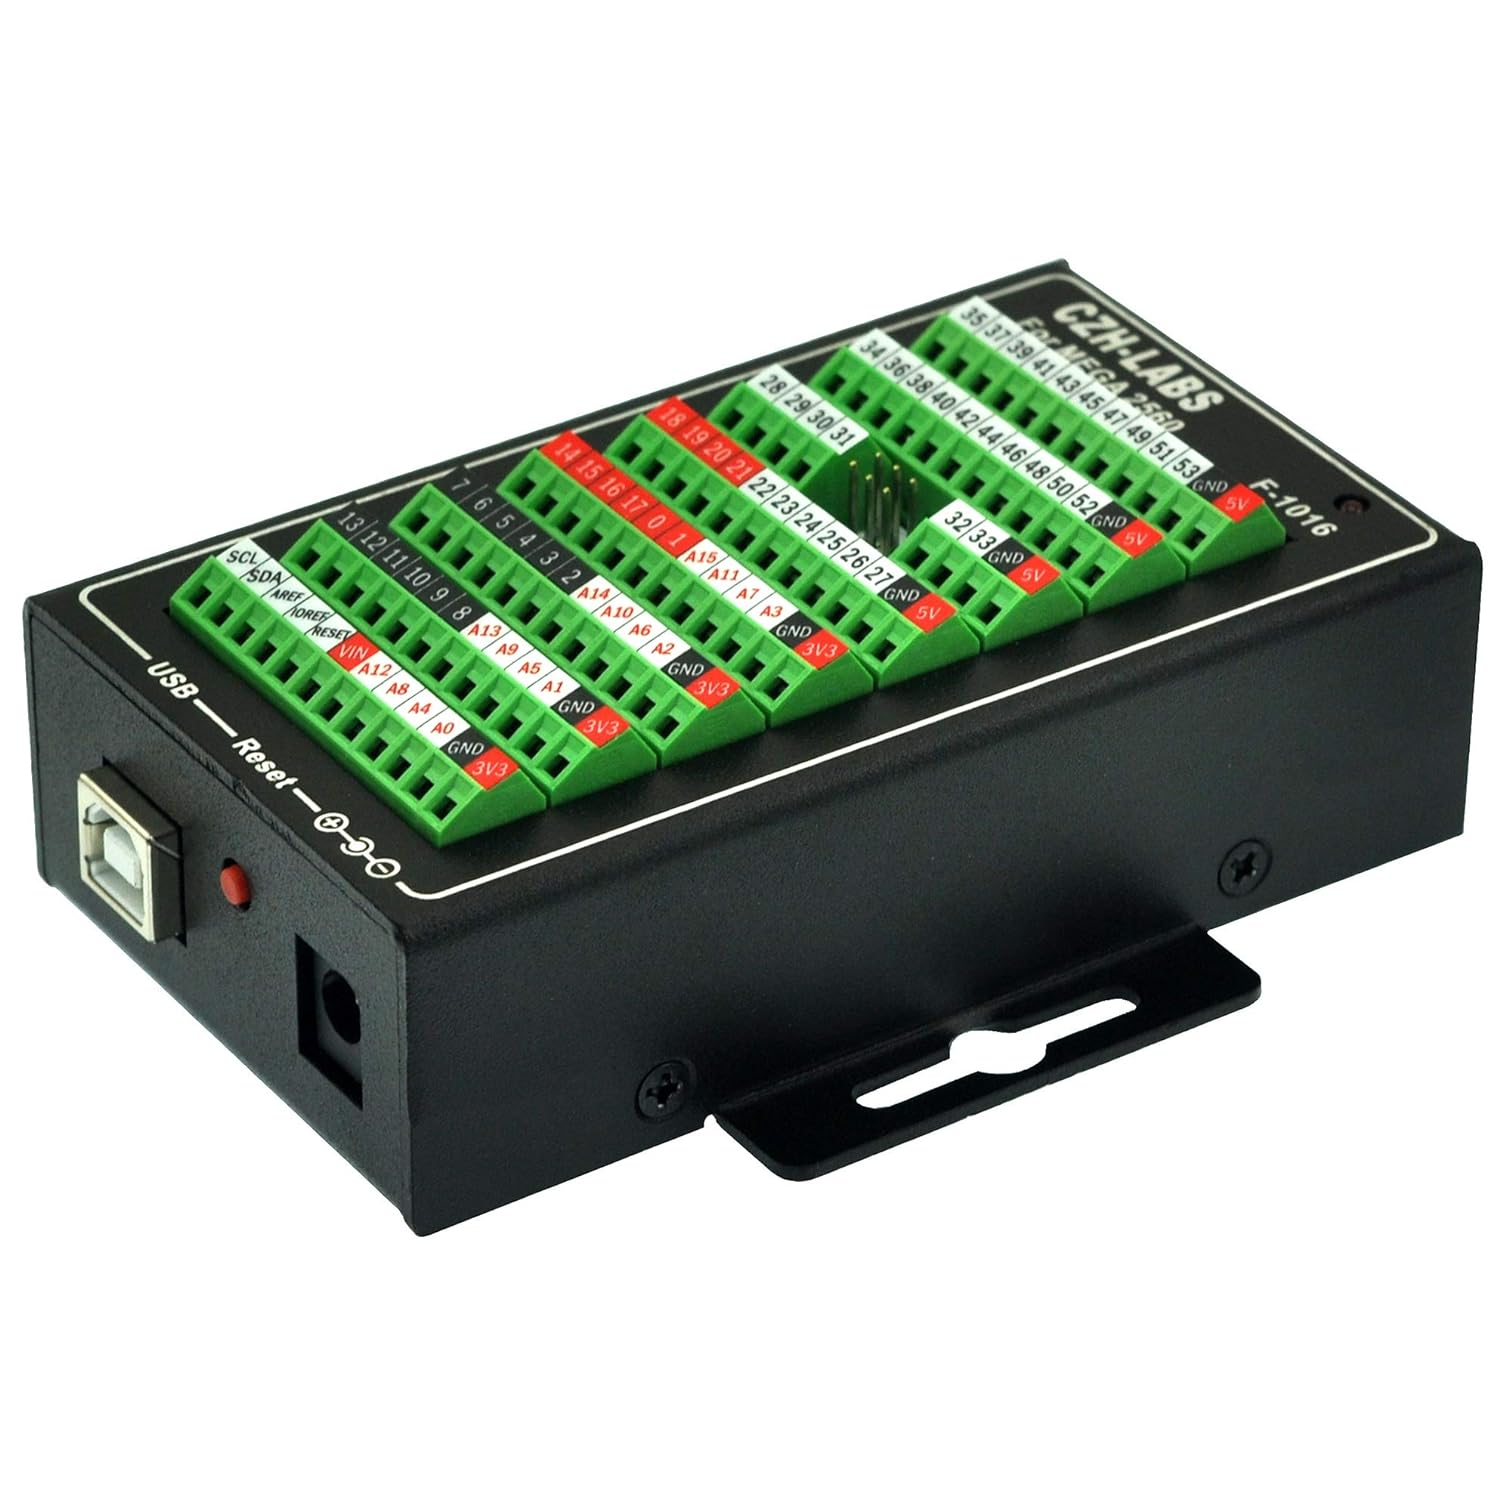
\includegraphics[
					height=60mm,
					width=\linewidth,
					keepaspectratio
				]{Resultados/Control/Arduino.png}
				\caption{Arduino con Shield}
			\end{figure}
		\end{column}
		\begin{column}{0.5\linewidth}
			\begin{figure}
				\centering
				
\includegraphics[
					height=60mm,
					width=\linewidth,
					keepaspectratio
				]{Resultados/Control/CPP.png}
				\caption{Programado en C++}
			\end{figure}
		\end{column}
	\end{columns}
		
\end{frame}

\begin{frame}
	\frametitle{Diagrama de clases del control}
	
	\begin{figure}
		\centering
		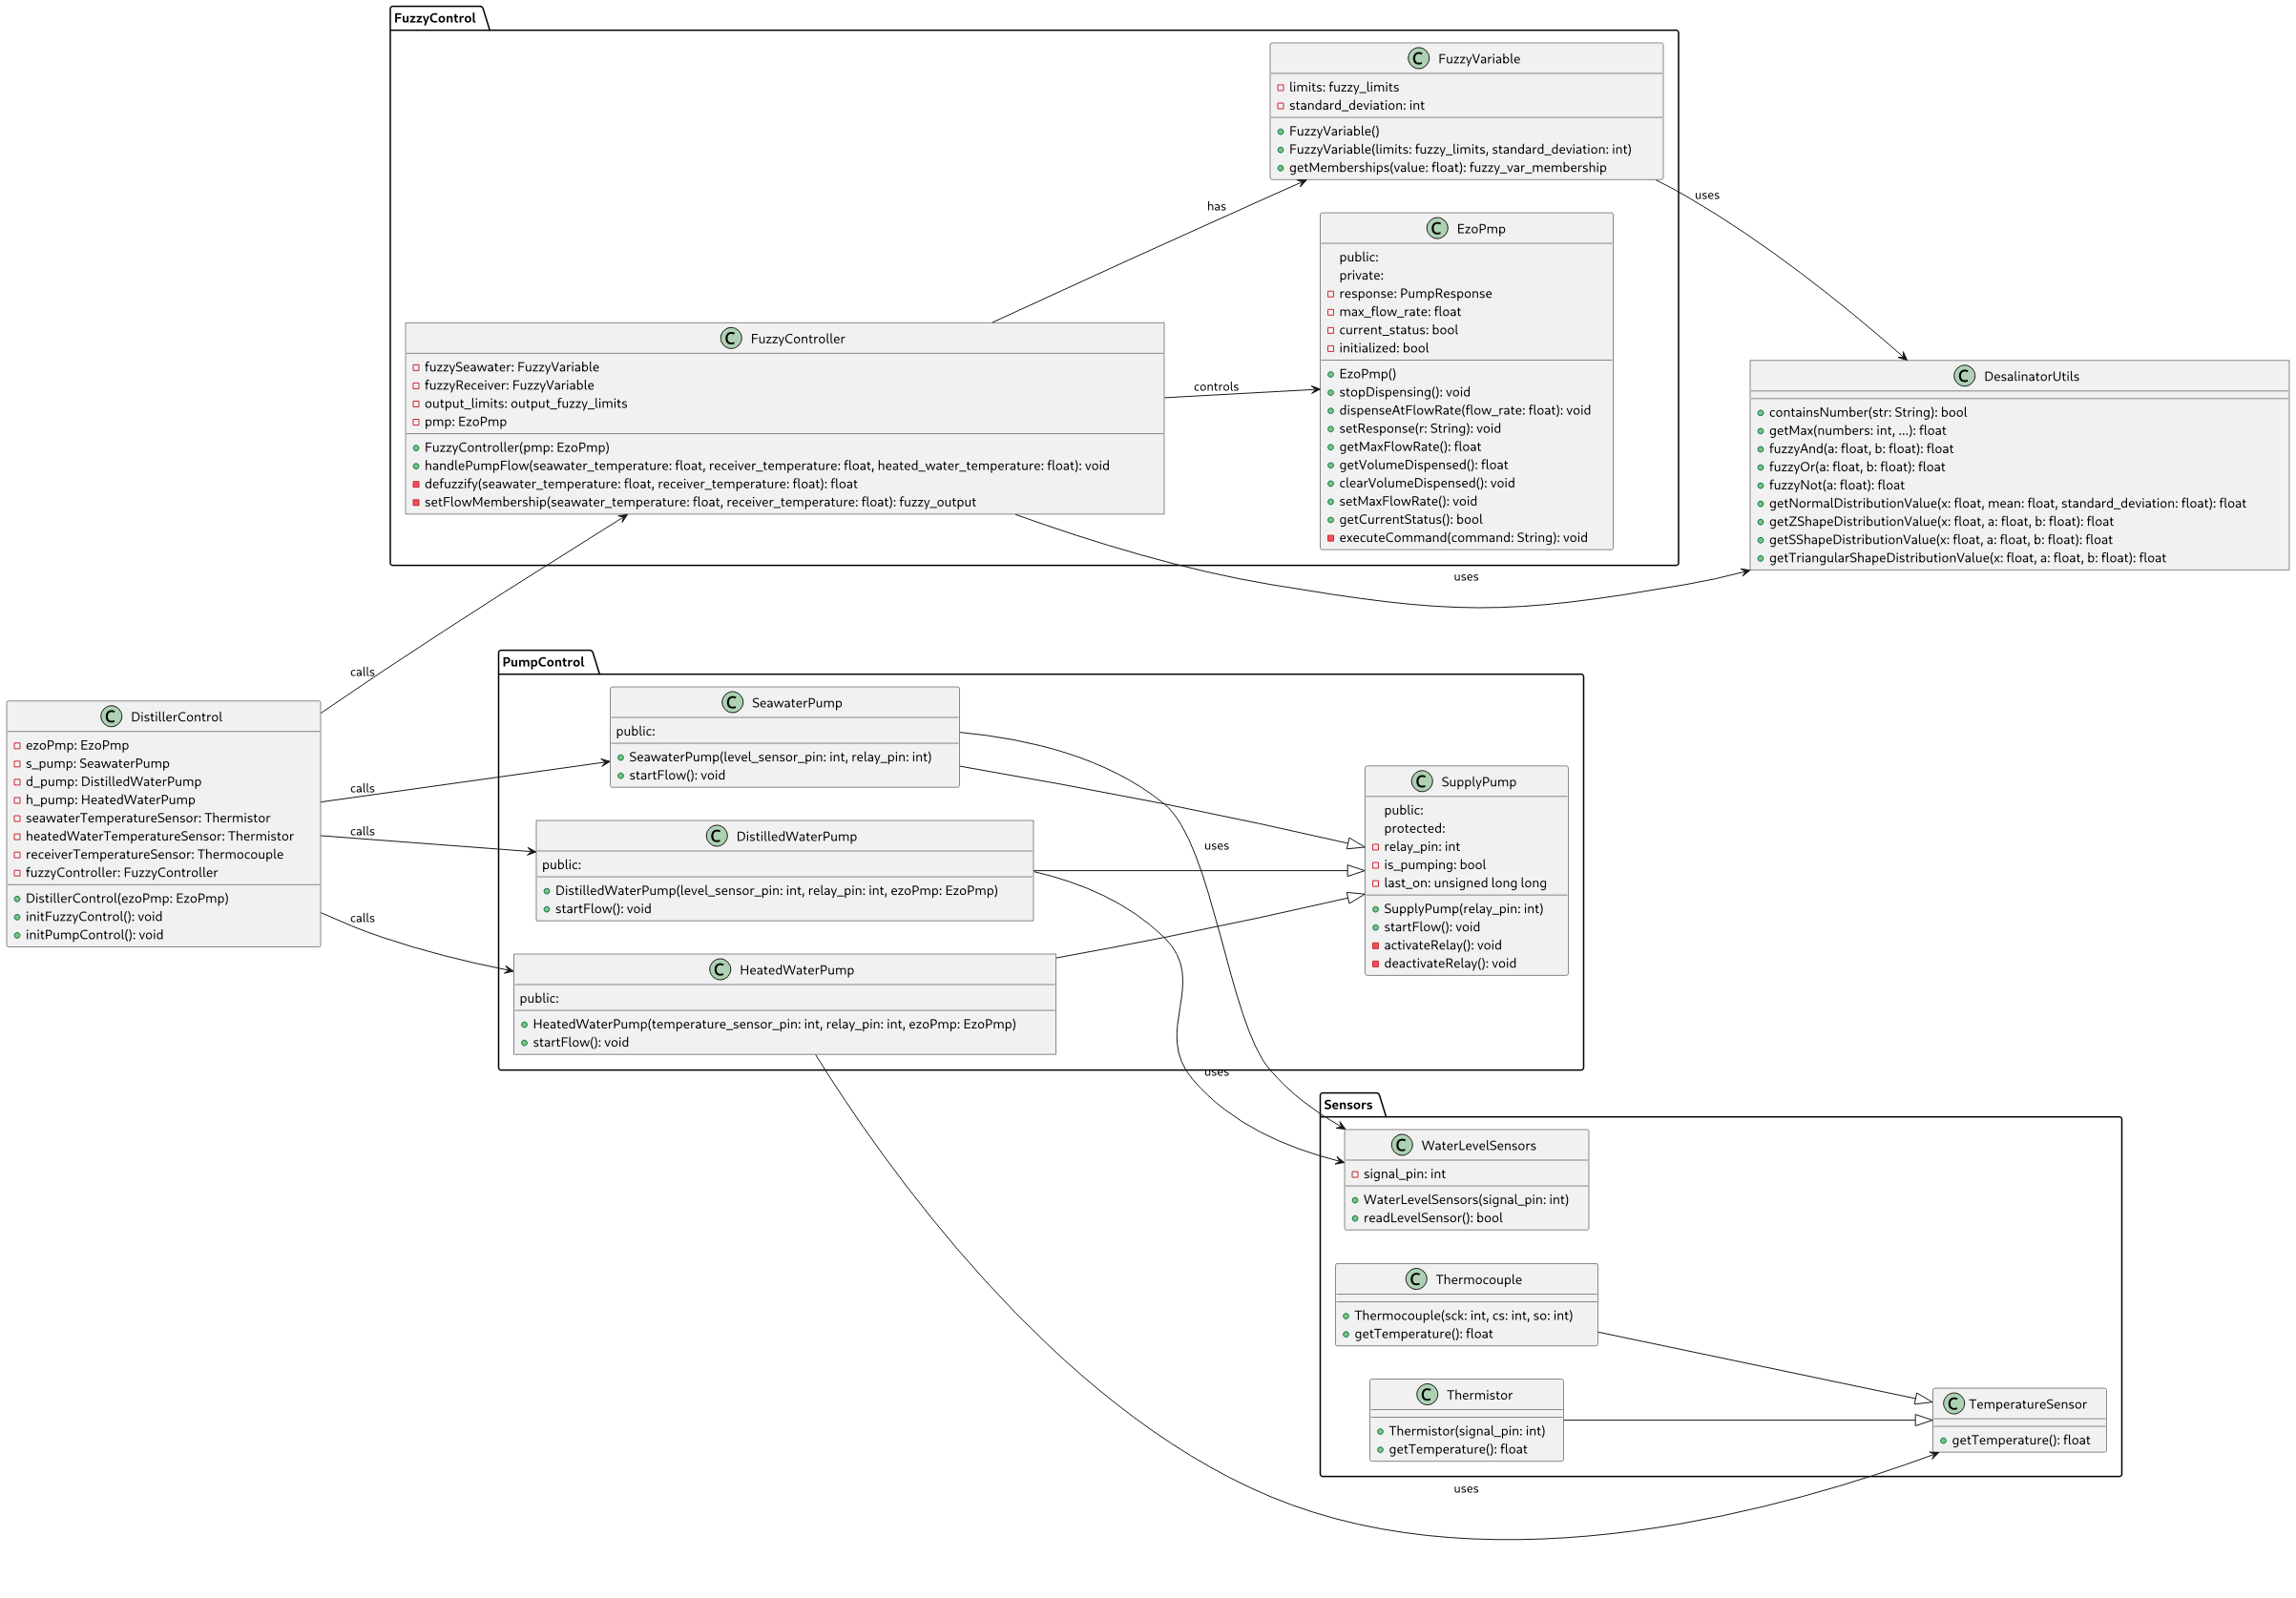
\includegraphics[
			height=70mm,
			width=\linewidth,
			keepaspectratio
		]{Resultados/Control/ClassDiagram.png}
		\caption{Diagrama de clases del control}
	\end{figure}
\end{frame}

\begin{frame}
	\frametitle{Control del sistema}
	\begin{columns}
		\begin{column}{0.5\linewidth}
			\textbf{Control del caudal}
		\end{column}
		\begin{column}{0.5\linewidth}
			\textbf{Control de los niveles de agua}
		\end{column}
	\end{columns}
	\vspace*{2mm}
	\begin{columns}
		\begin{column}{0.5\linewidth}
			Control difuso encargado de regular el flujo de agua que fluye hacia el recibidor solar. Usa sensores de temperatura y controla la bomba EZO-PMP.
		\end{column}
		\begin{column}{0.5\linewidth}
			Control On/Off encargado de llenar y vaciar los submódulos del módulo de reaprovechamiento térmico y bombeo. Usa sensores de nivel y tiempo transcurrido para tomar decisiones.
		\end{column}
	\end{columns}
\end{frame}

\begin{frame}
	\frametitle{Control difuso}
	\vspace*{2mm}
	\begin{columns}
		\begin{column}{0.5\linewidth}
			\begin{figure}
				\centering
				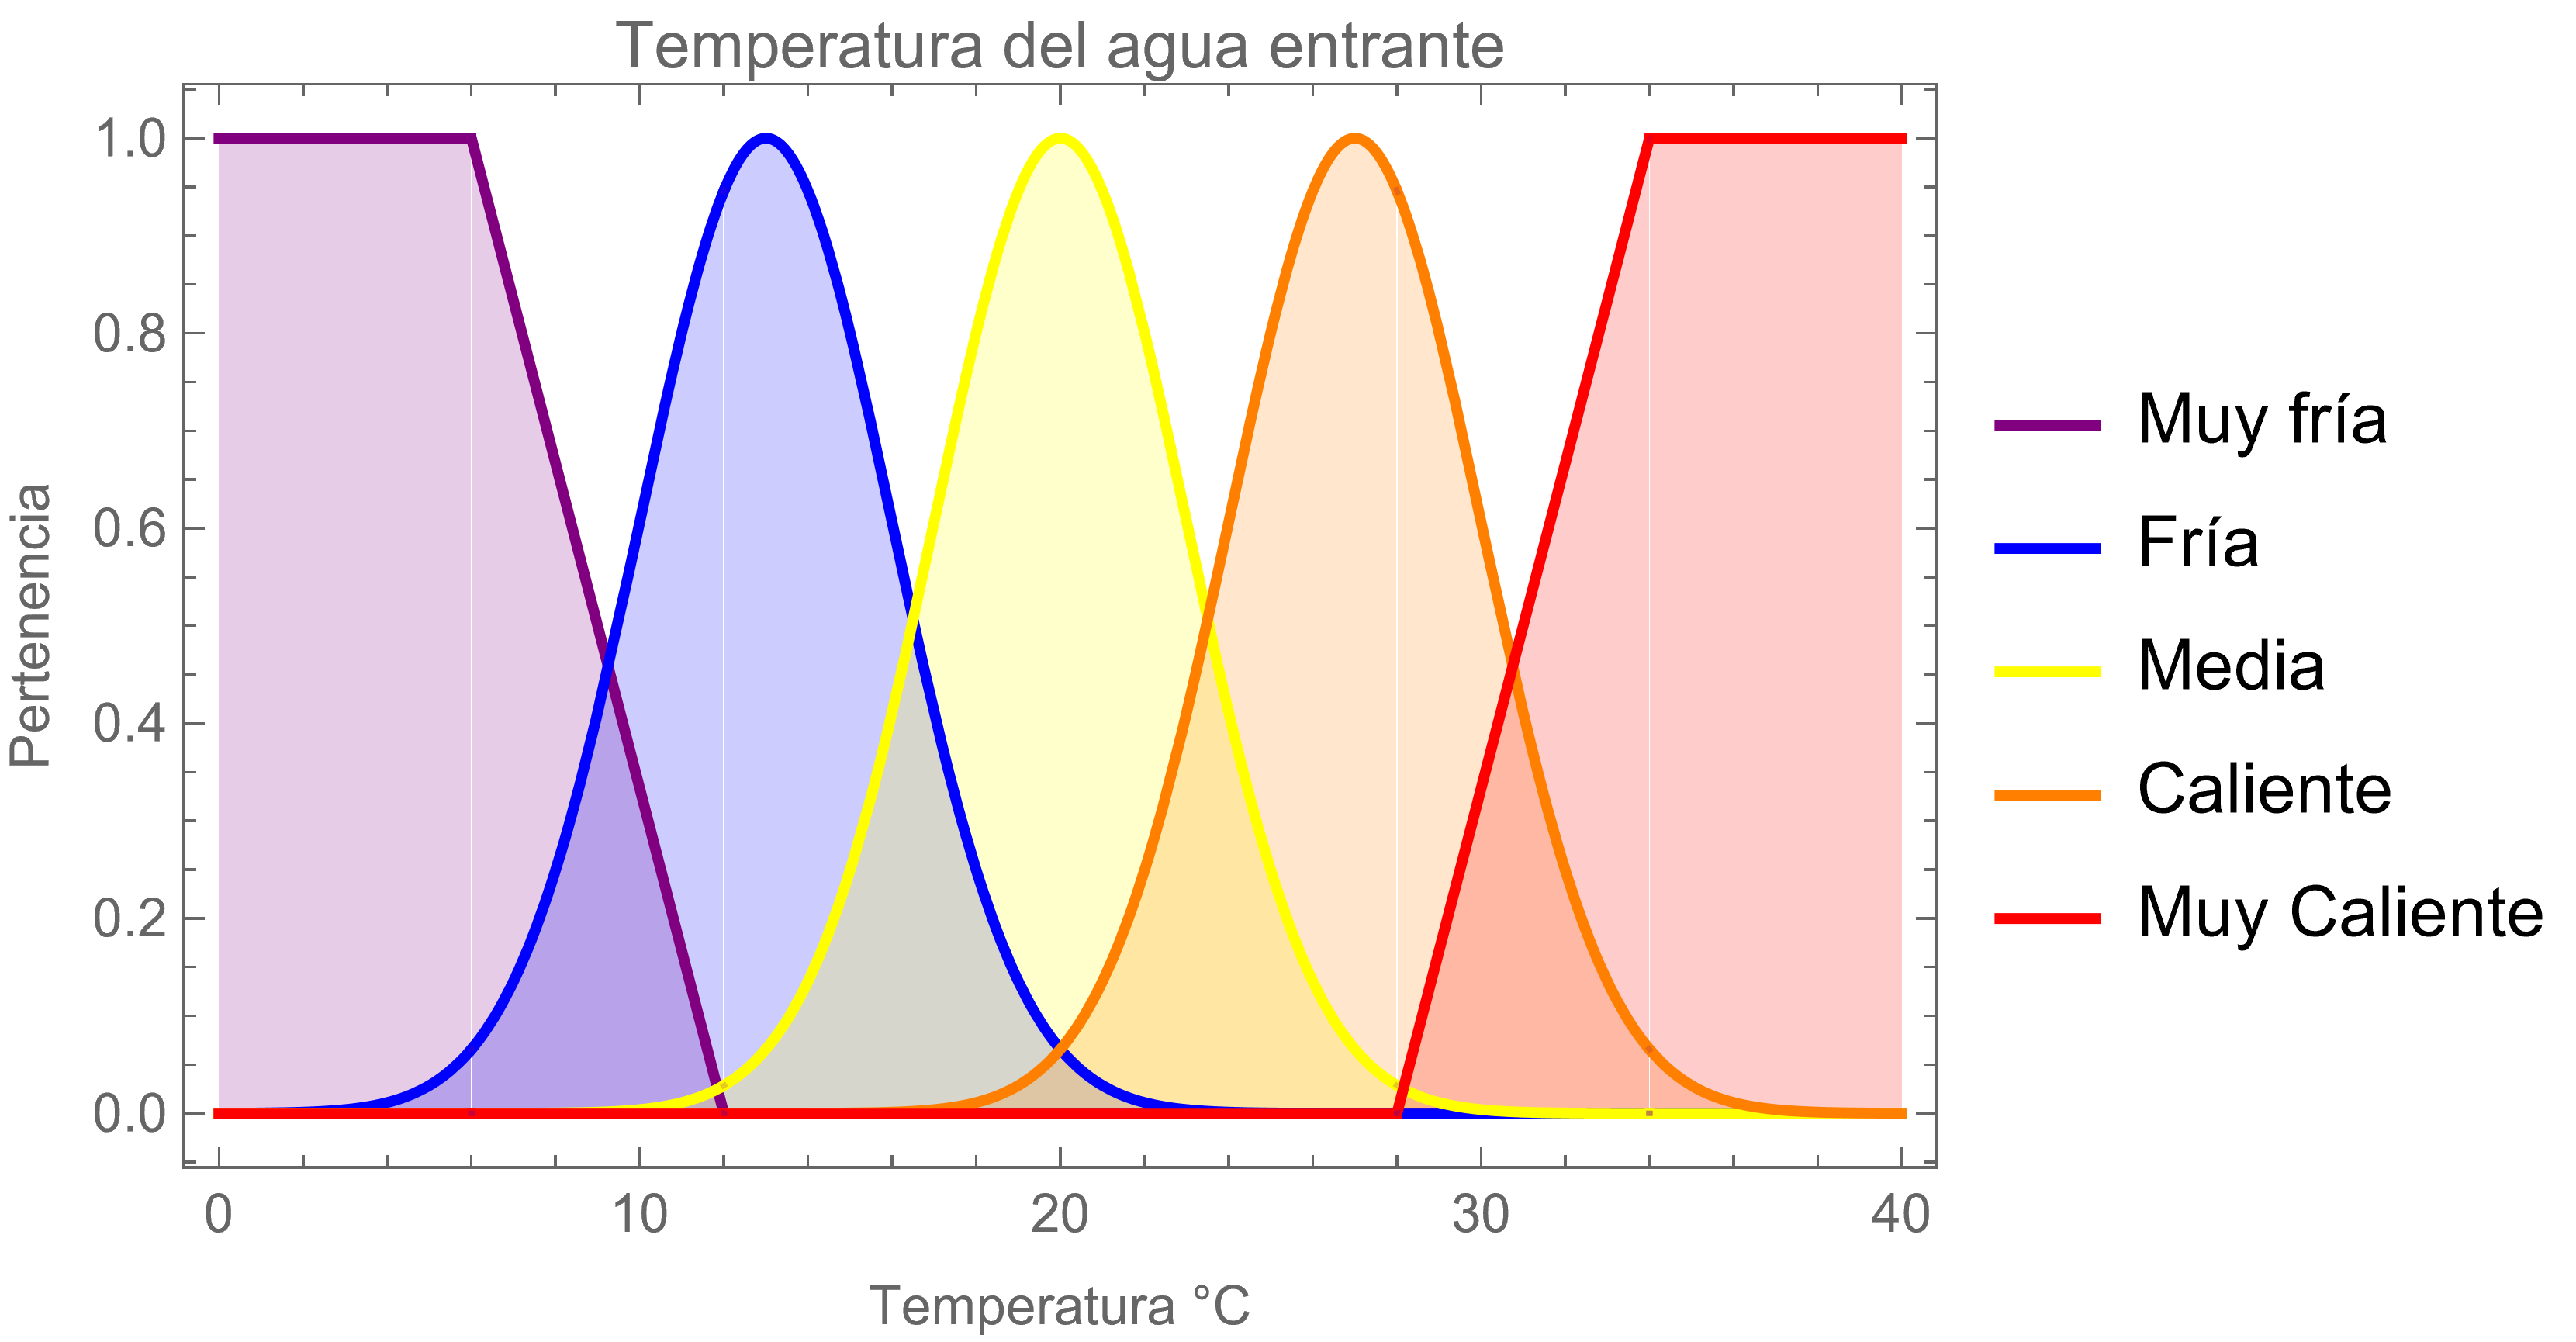
\includegraphics[
					height=70mm,
					width=\linewidth,
					keepaspectratio
				]{Resultados/Control/SeawaterTemperature.png}
				\caption{Universo de discurso y funciones de membresía de la temperatura del agua de mar entrante}
			\end{figure}
		\end{column}
		\begin{column}{0.5\linewidth}
			\begin{figure}
				\centering
				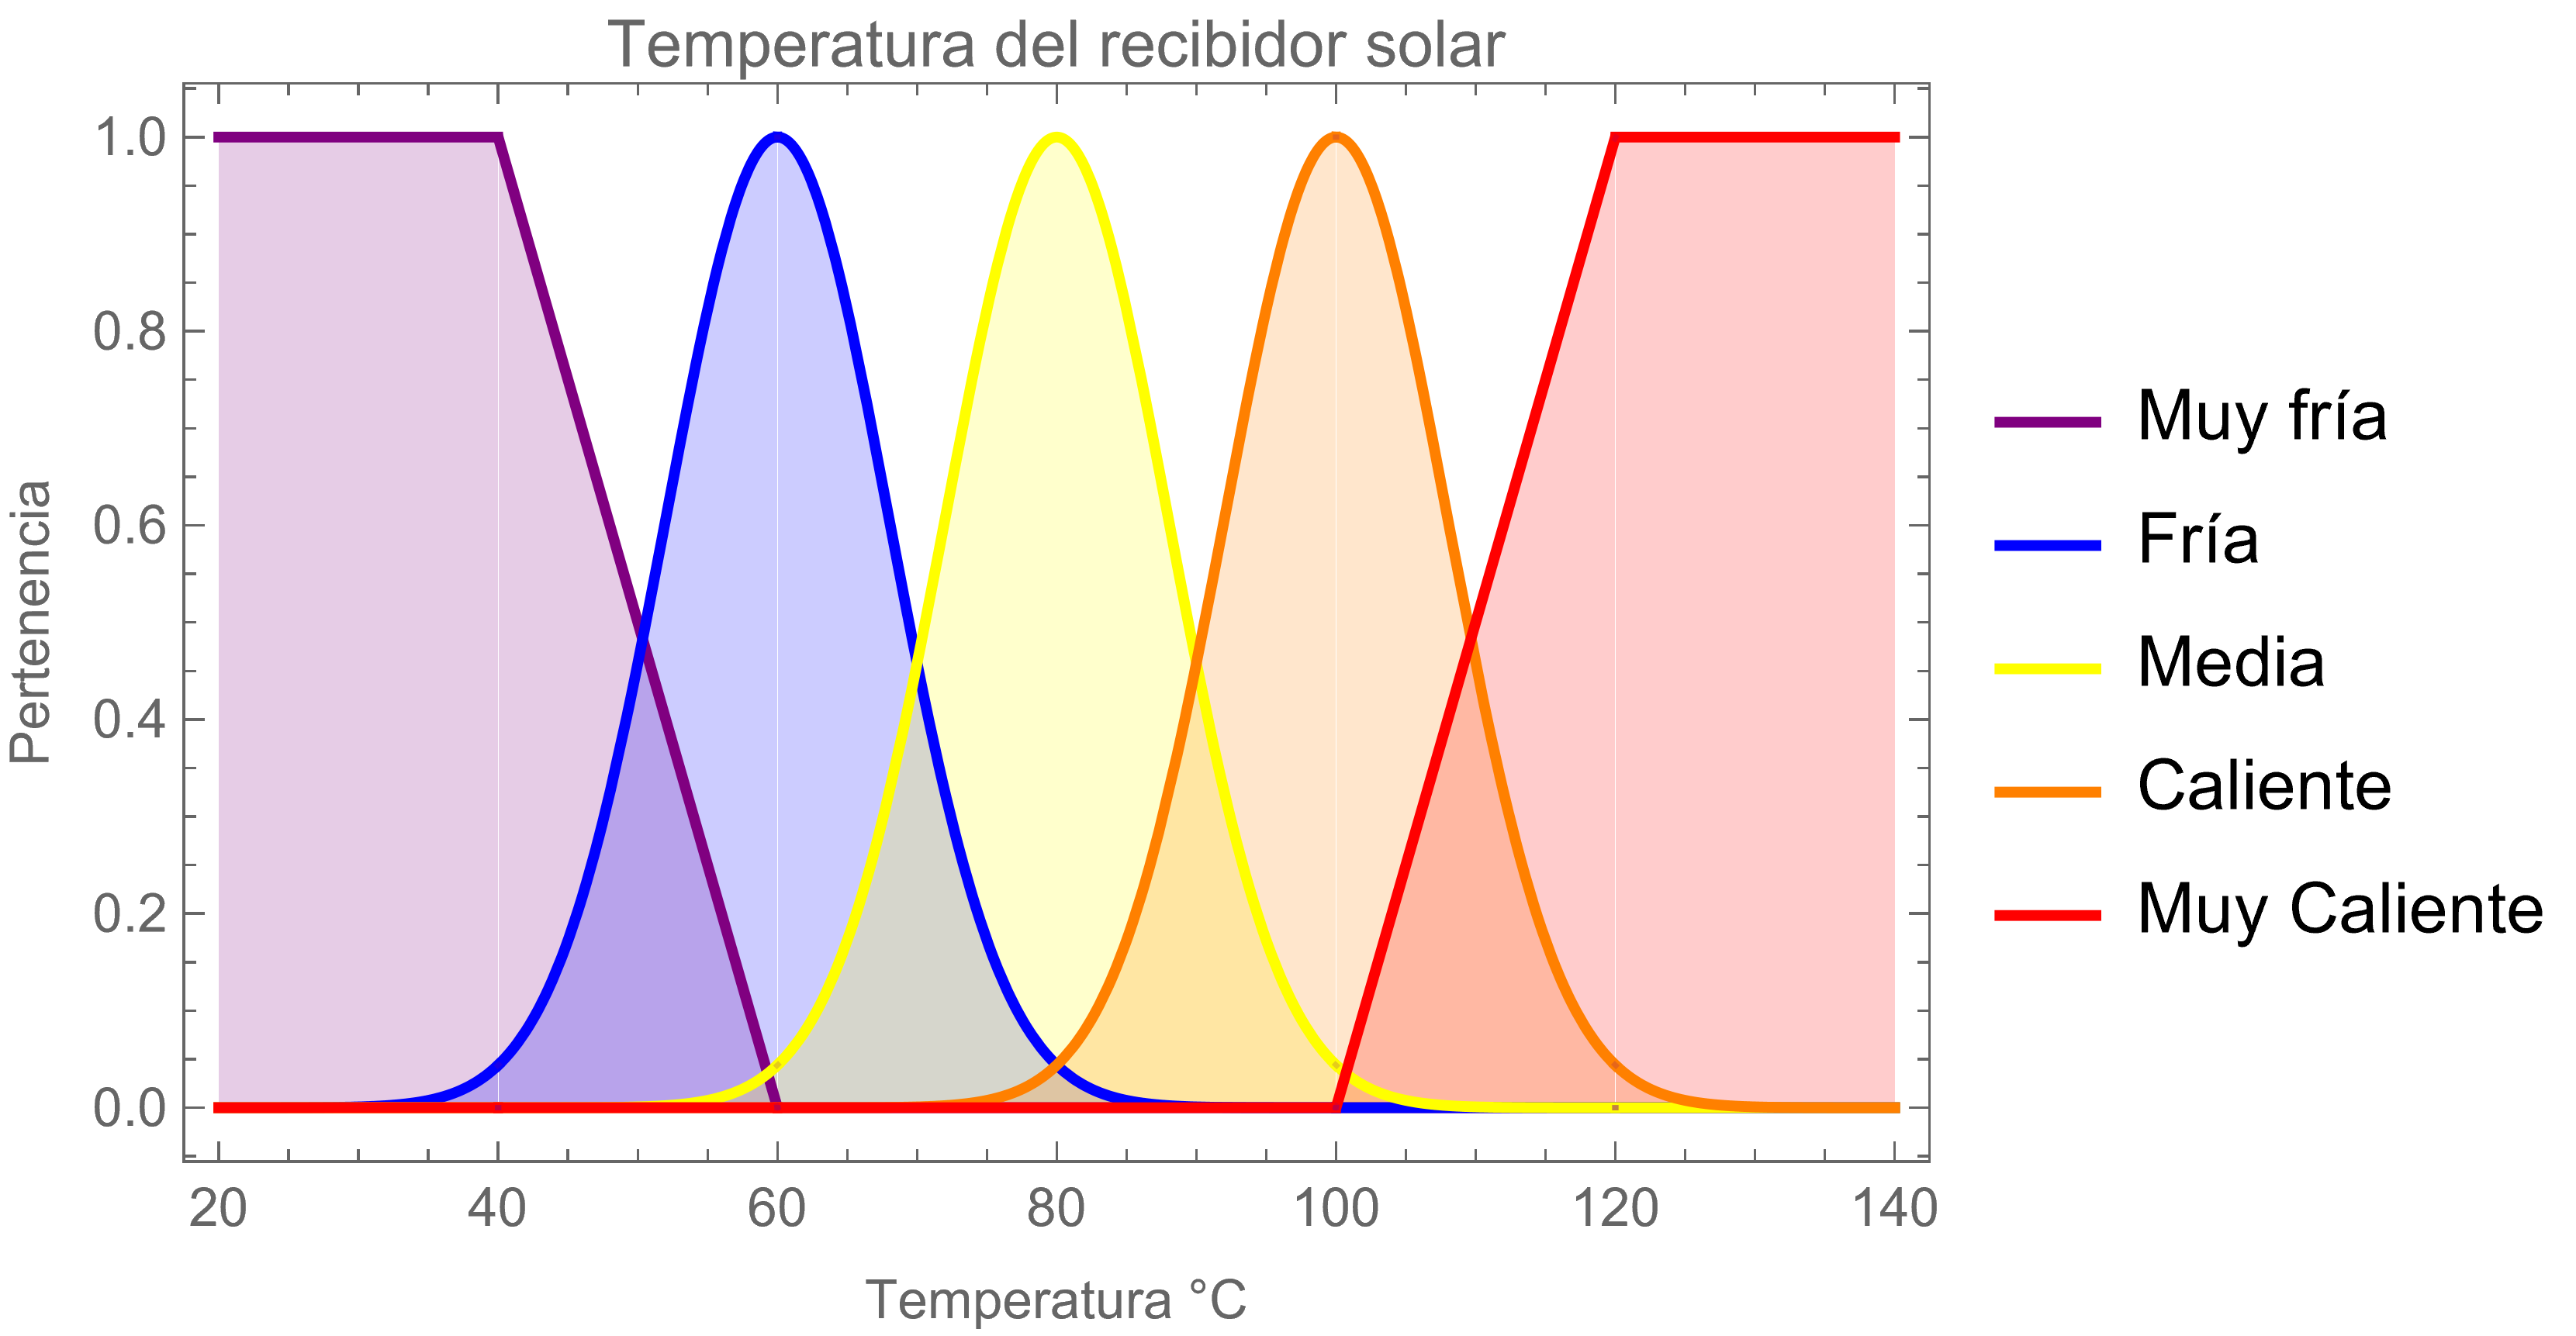
\includegraphics[
					height=70mm,
					width=\linewidth,
					keepaspectratio
				]{Resultados/Control/SolarReceiverTemperature.png}
				\caption{Universo de discurso y funciones de membresía de la temperatura del recibidor solar}
			\end{figure}
		\end{column}
	\end{columns}
\end{frame}

\begin{frame}
	\frametitle{Control difuso}
	
	\begin{figure}
		\centering
		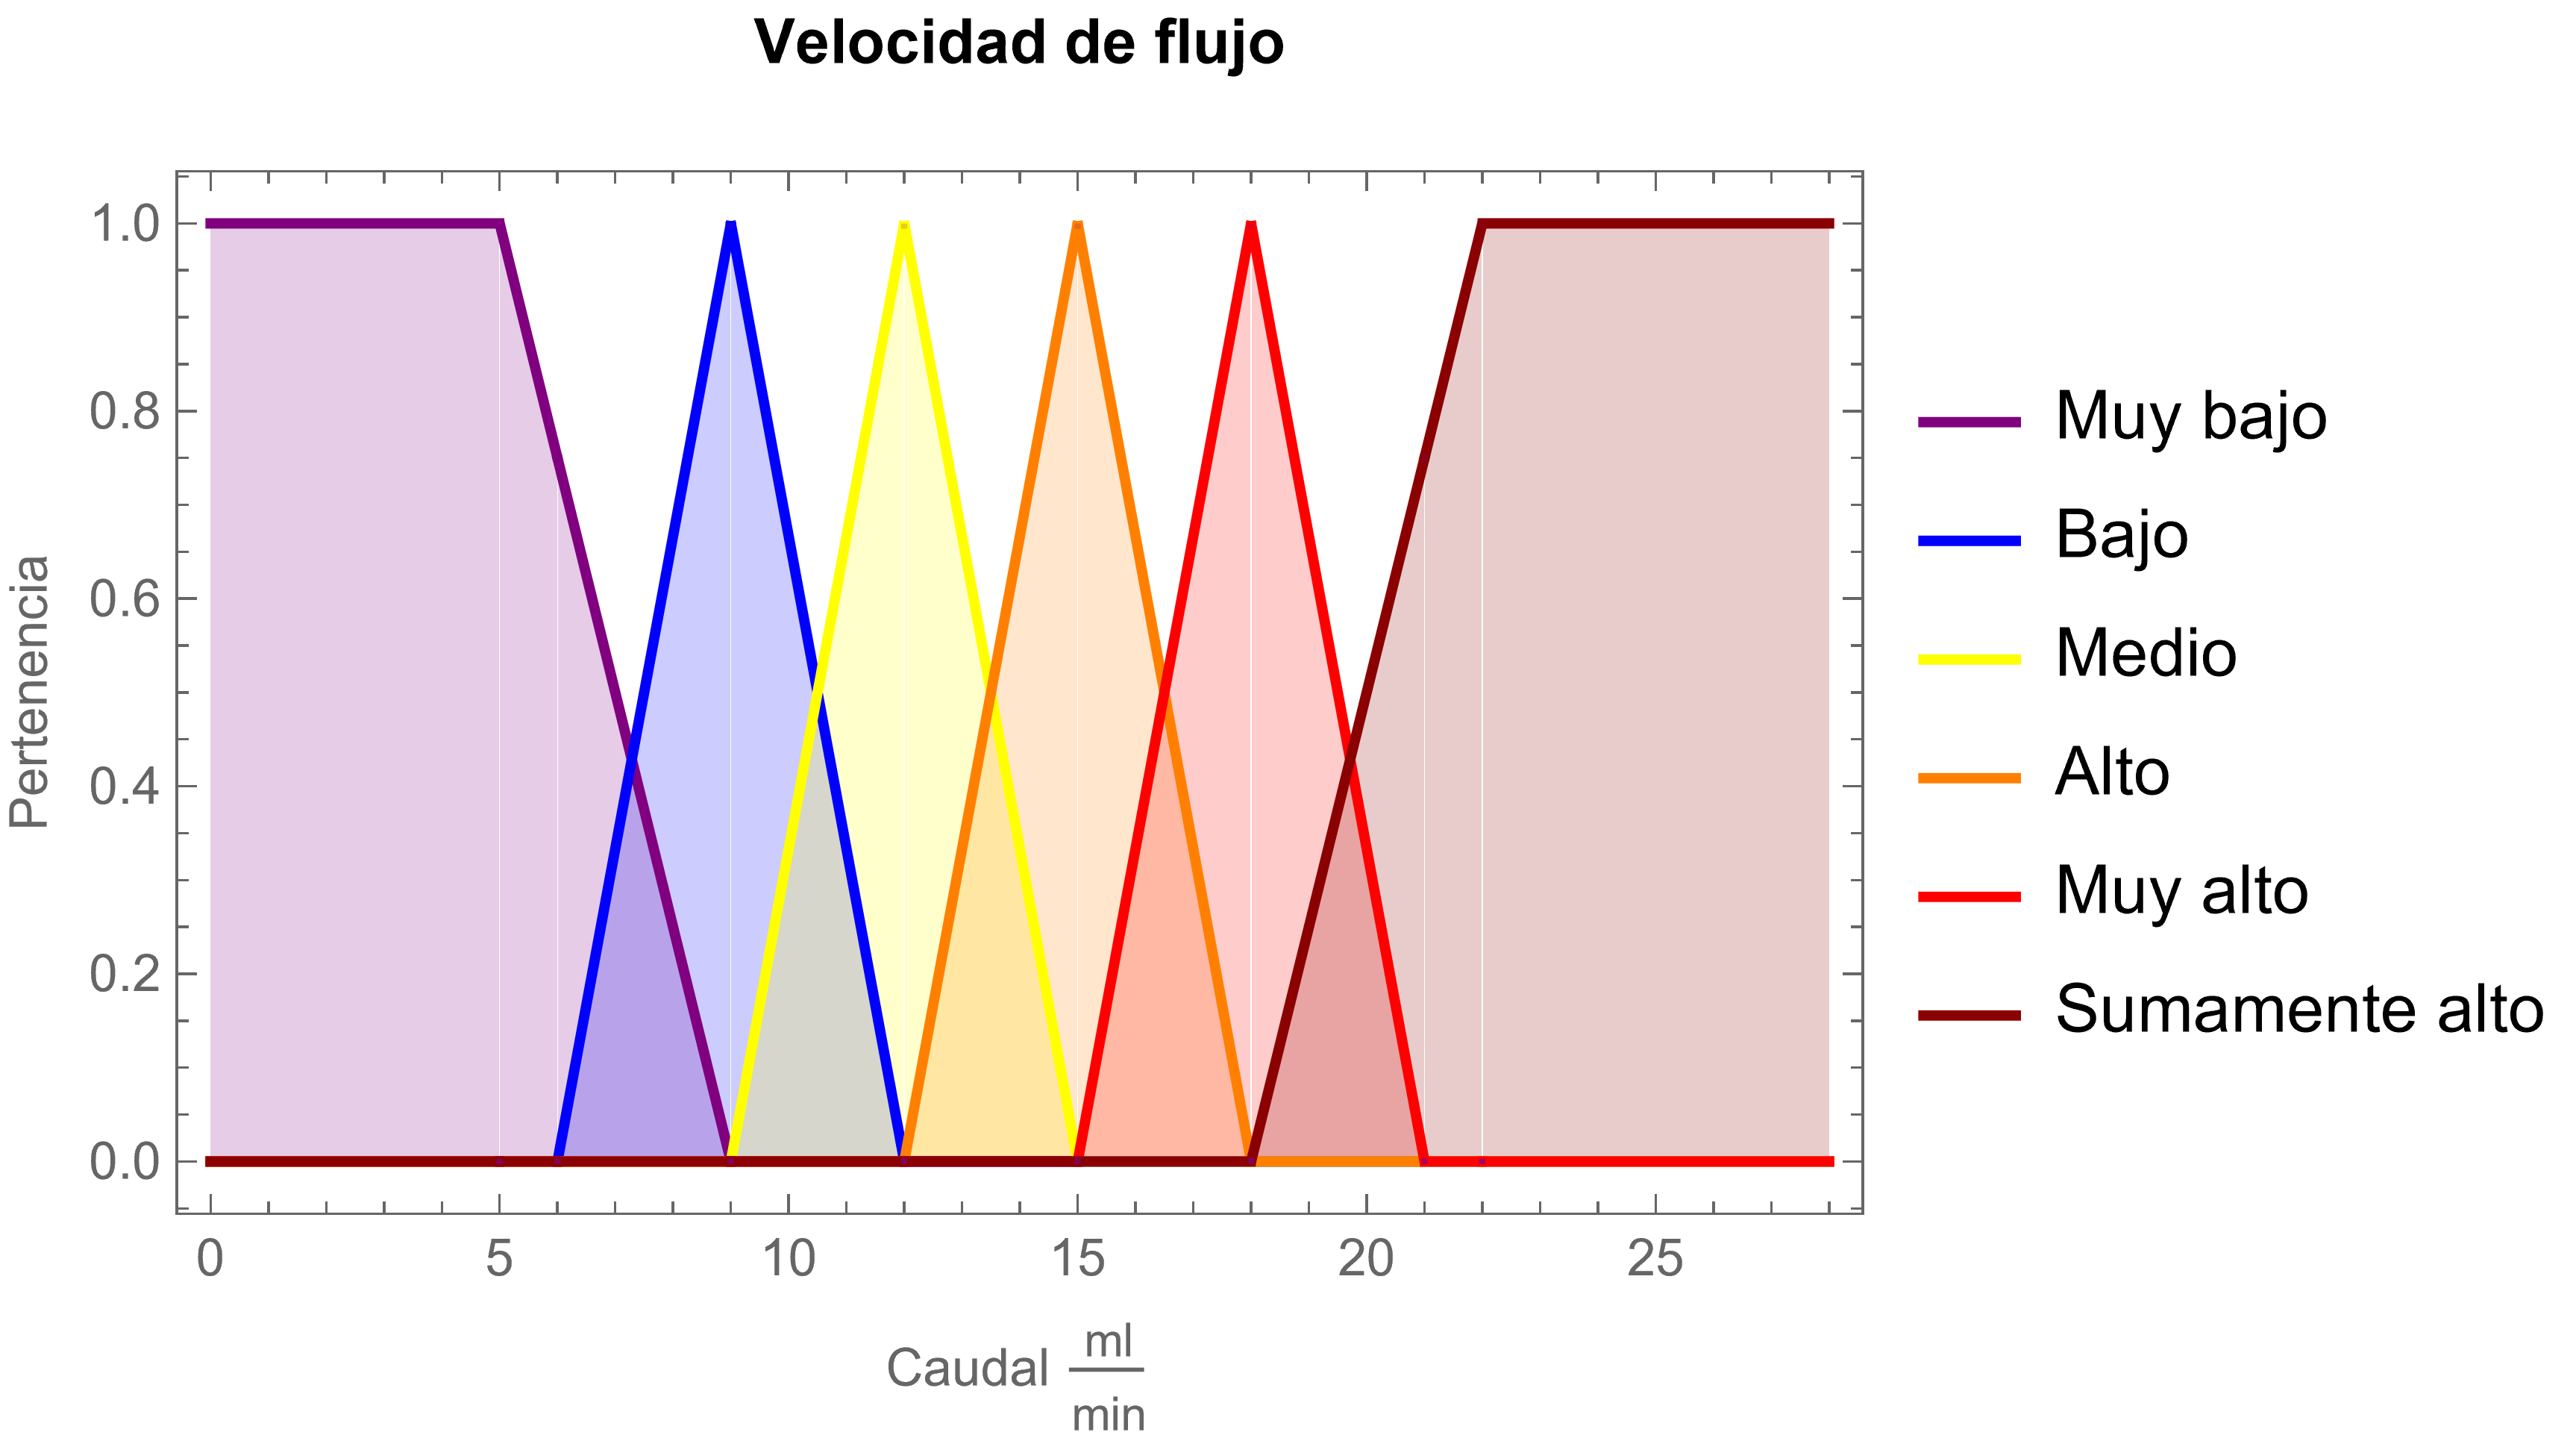
\includegraphics[
			height=60mm,
			width=\linewidth,
			keepaspectratio
		]{Resultados/Control/FlowVelocity.png}
		\caption{Universo de discurso y funciones de membresía del caudal de agua}
	\end{figure}
\end{frame}

\subsection{Construcción}
\begin{frame}
	\frametitle{Construcción e integración}
	\begin{columns}
		\begin{column}{0.5\linewidth}
			\begin{figure}
				\centering
				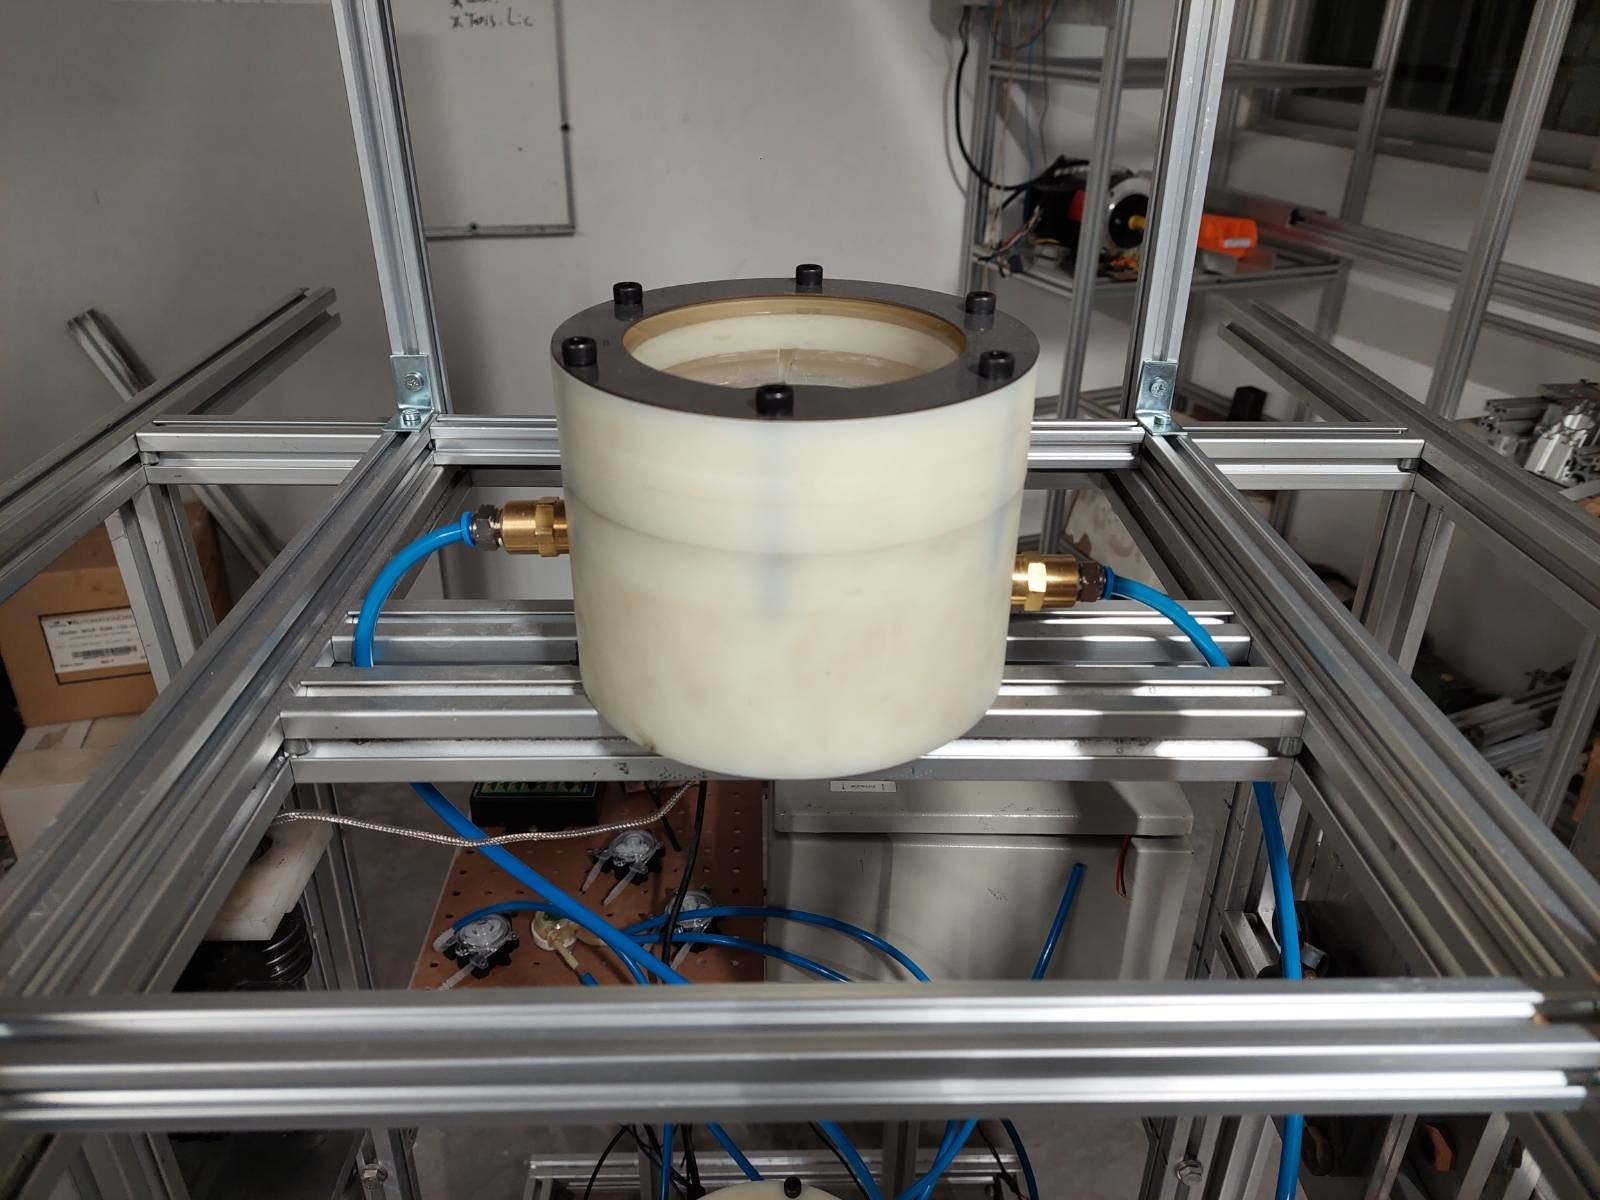
\includegraphics[
					height=70mm,
					width=\linewidth,
					keepaspectratio
				]{Resultados/Construcción/SolarModule.jpeg}
				\caption{Módulo de concentración solar integrado al seguidor solar}
			\end{figure}
		\end{column}
		\begin{column}{0.5\linewidth}
			\begin{figure}
				\centering
				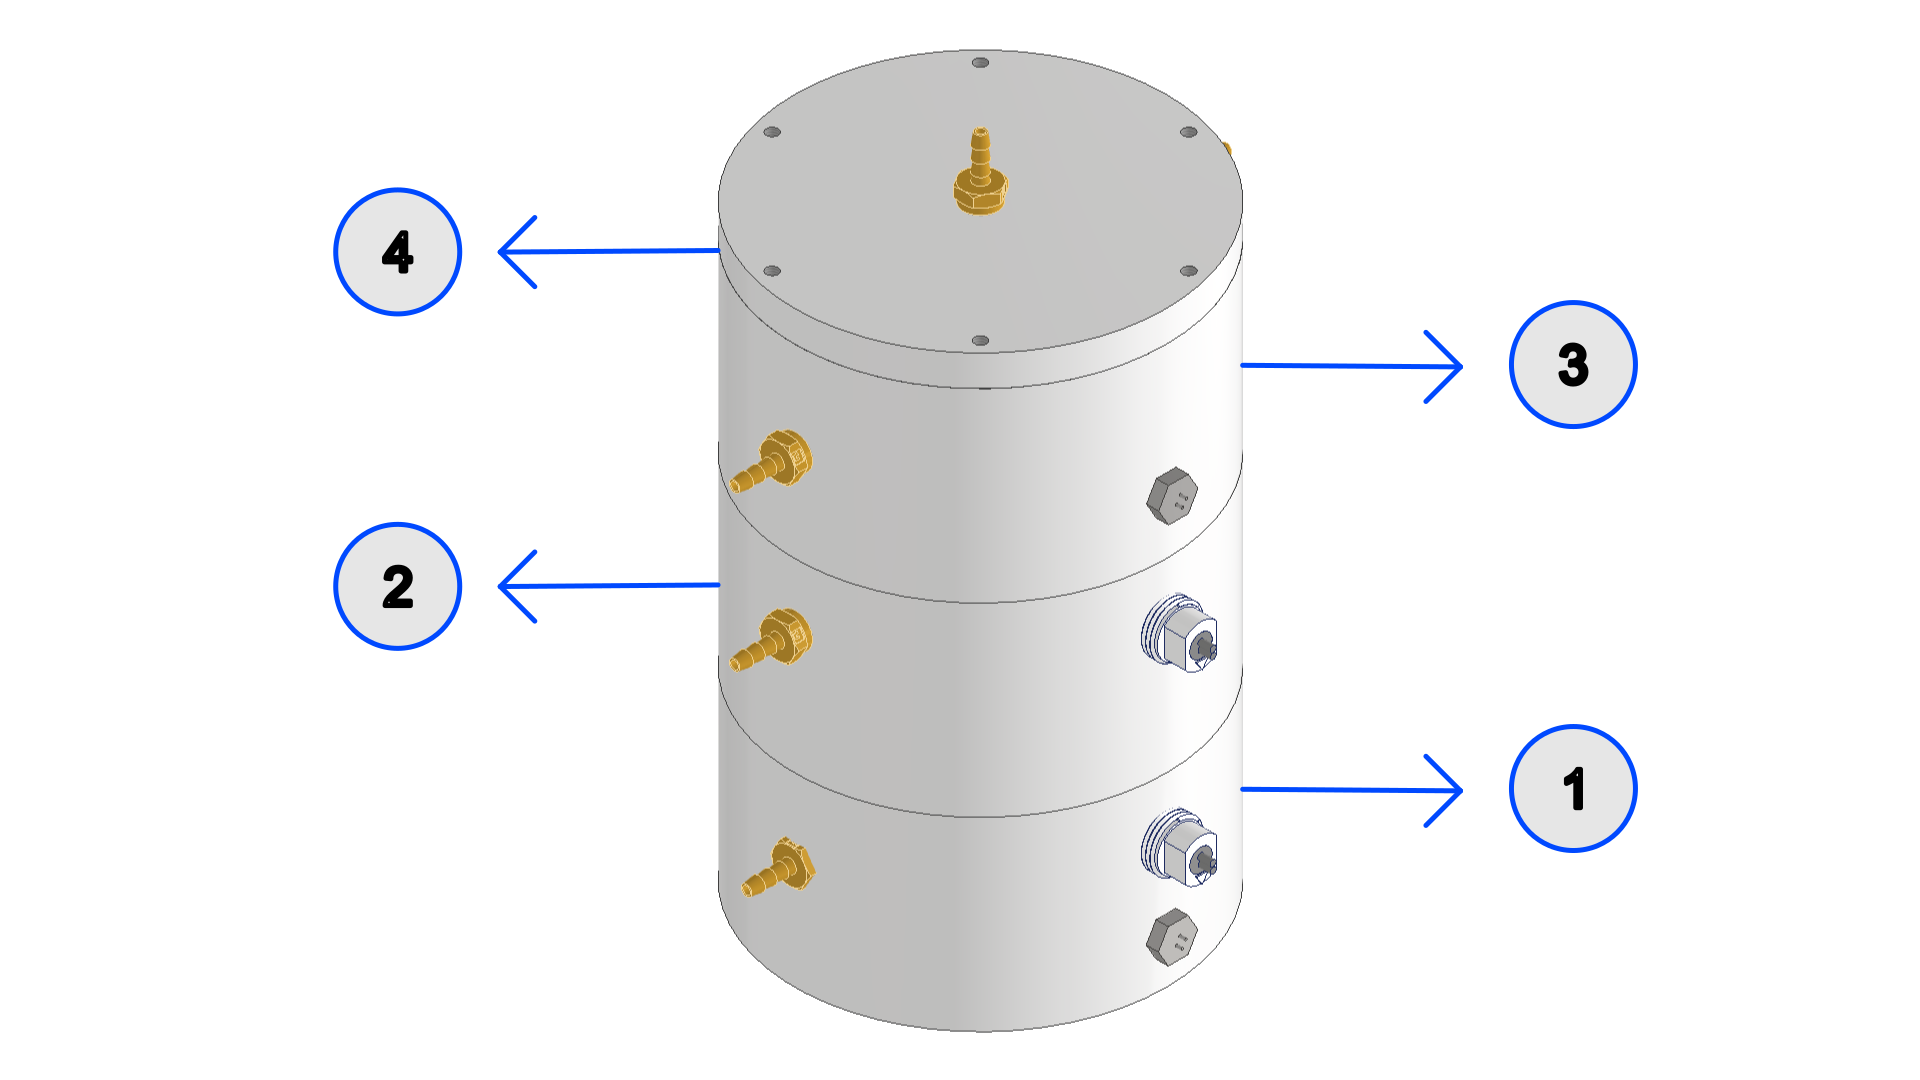
\includegraphics[
					height=60mm,
					width=\linewidth,
					keepaspectratio
				]{Resultados/Construcción/WaterModule.png}
				\caption{Módulo de reaprovechamiento térmico y bombeo}
			\end{figure}
		\end{column}
	\end{columns}
\end{frame}

\begin{frame}
	\frametitle{Preparación}
	\begin{columns}
		\begin{column}{0.5\linewidth}
			\begin{figure}
				\centering
				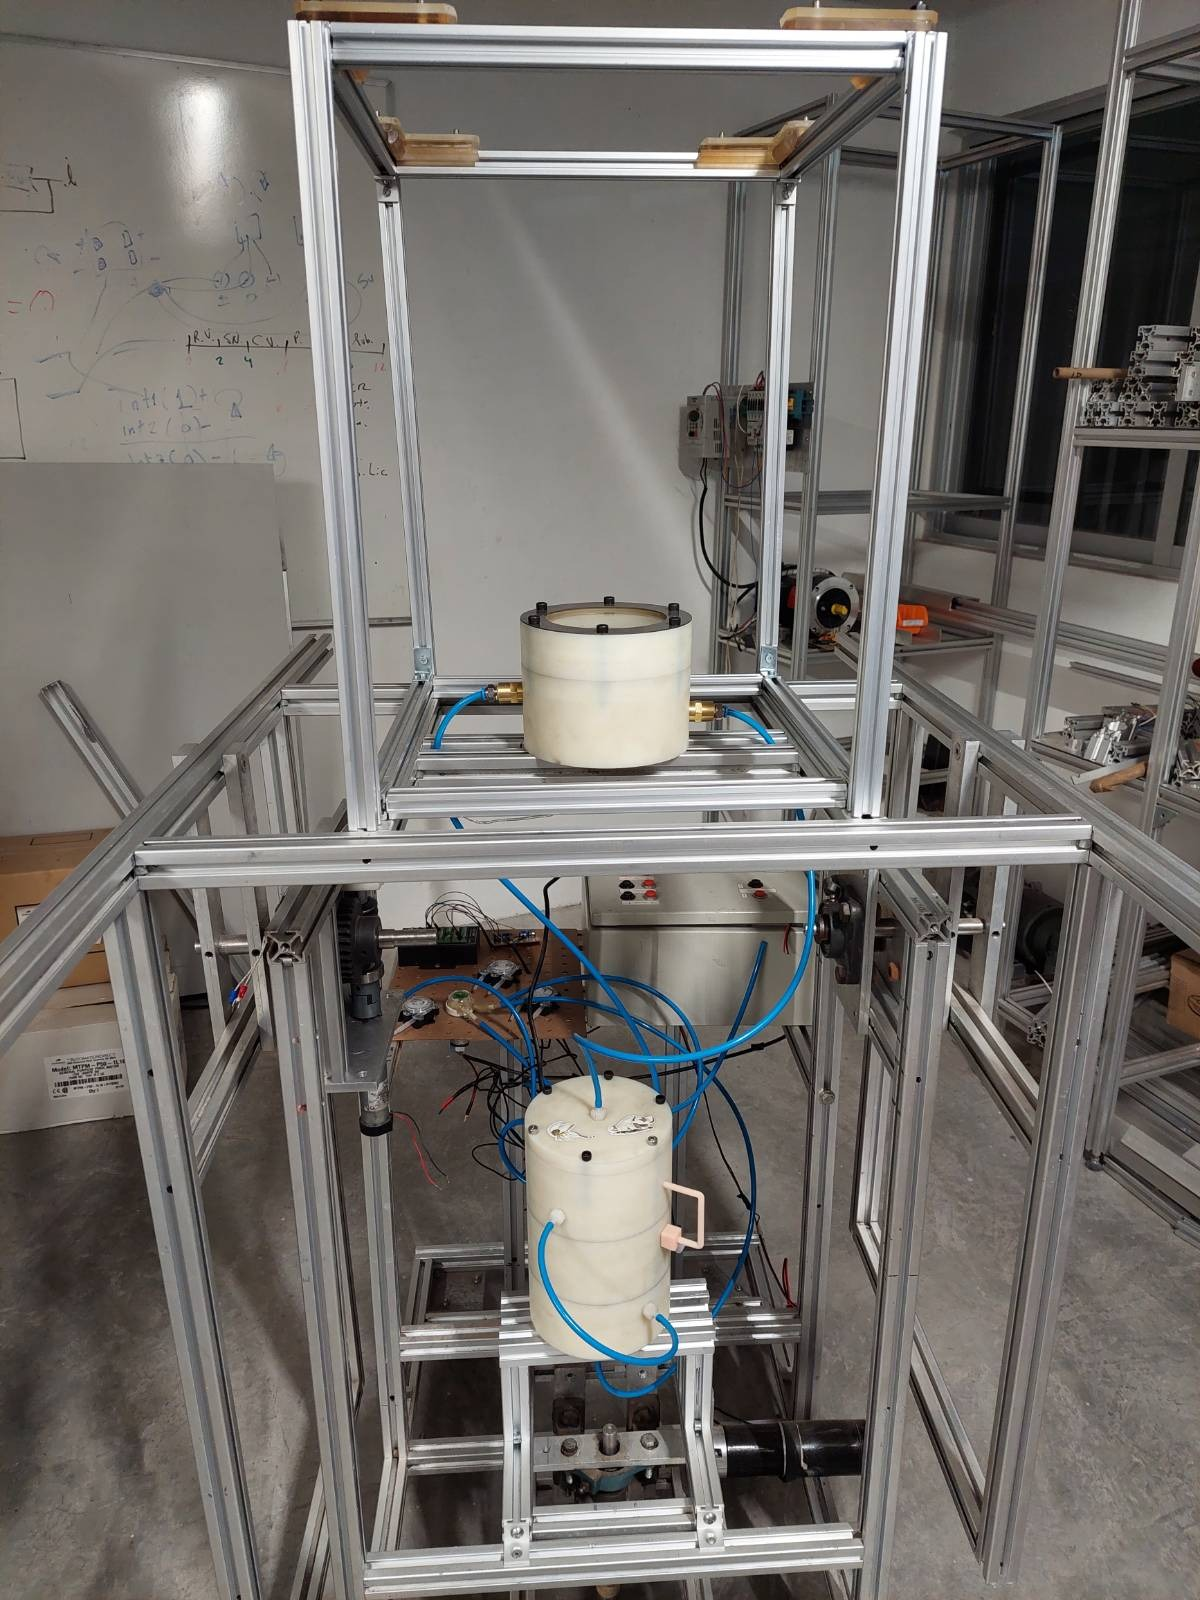
\includegraphics[
					height=70mm,
					width=\linewidth,
					keepaspectratio
				]{Resultados/Construcción/Completo.jpeg}
				\caption{Ensamble completo}
			\end{figure}
		\end{column}
		\begin{column}{0.5\linewidth}
			\begin{figure}
				\centering
				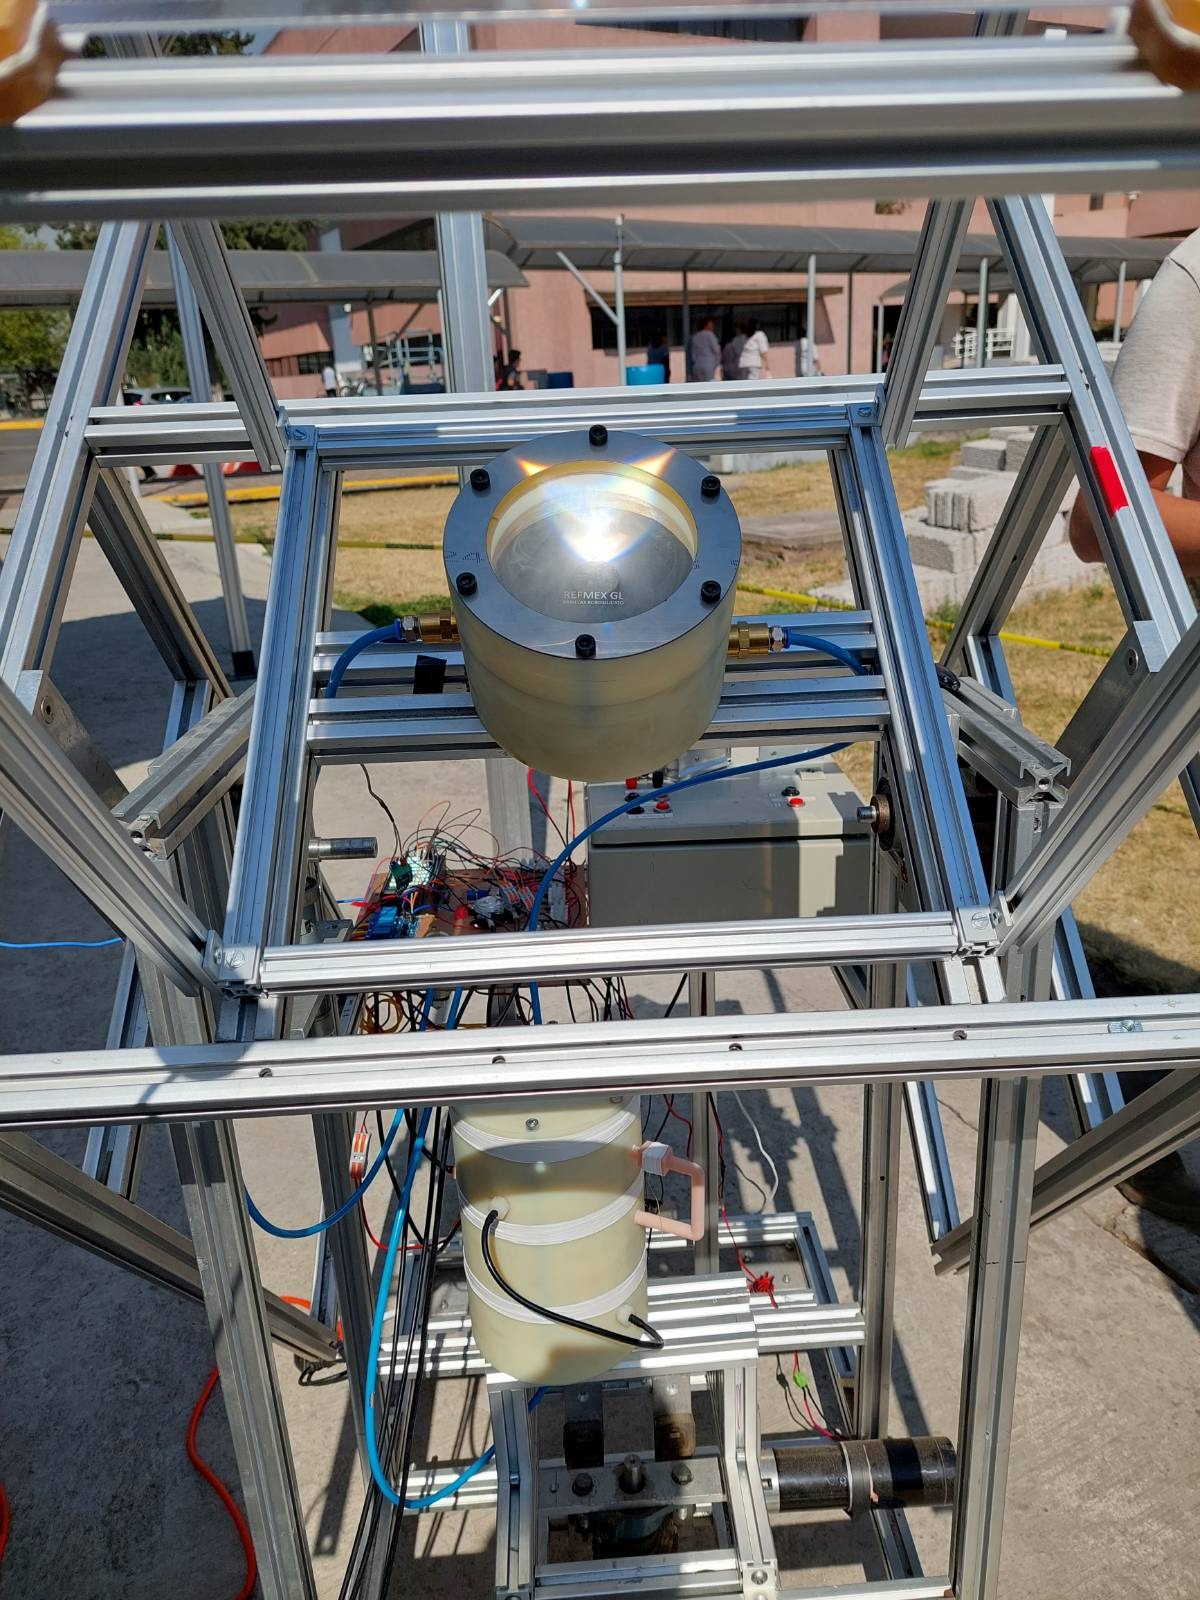
\includegraphics[
					height=70mm,
					width=\linewidth,
					keepaspectratio
				]{Resultados/Discusión/Alineación.jpeg}
				\caption{Concentración solar sobre el recibidor}
			\end{figure}
		\end{column}
	\end{columns}
\end{frame}

\begin{frame}
	\frametitle{Puesta en marcha}
	\begin{columns}
		\begin{column}{0.5\linewidth}
			\begin{figure}
				\centering
				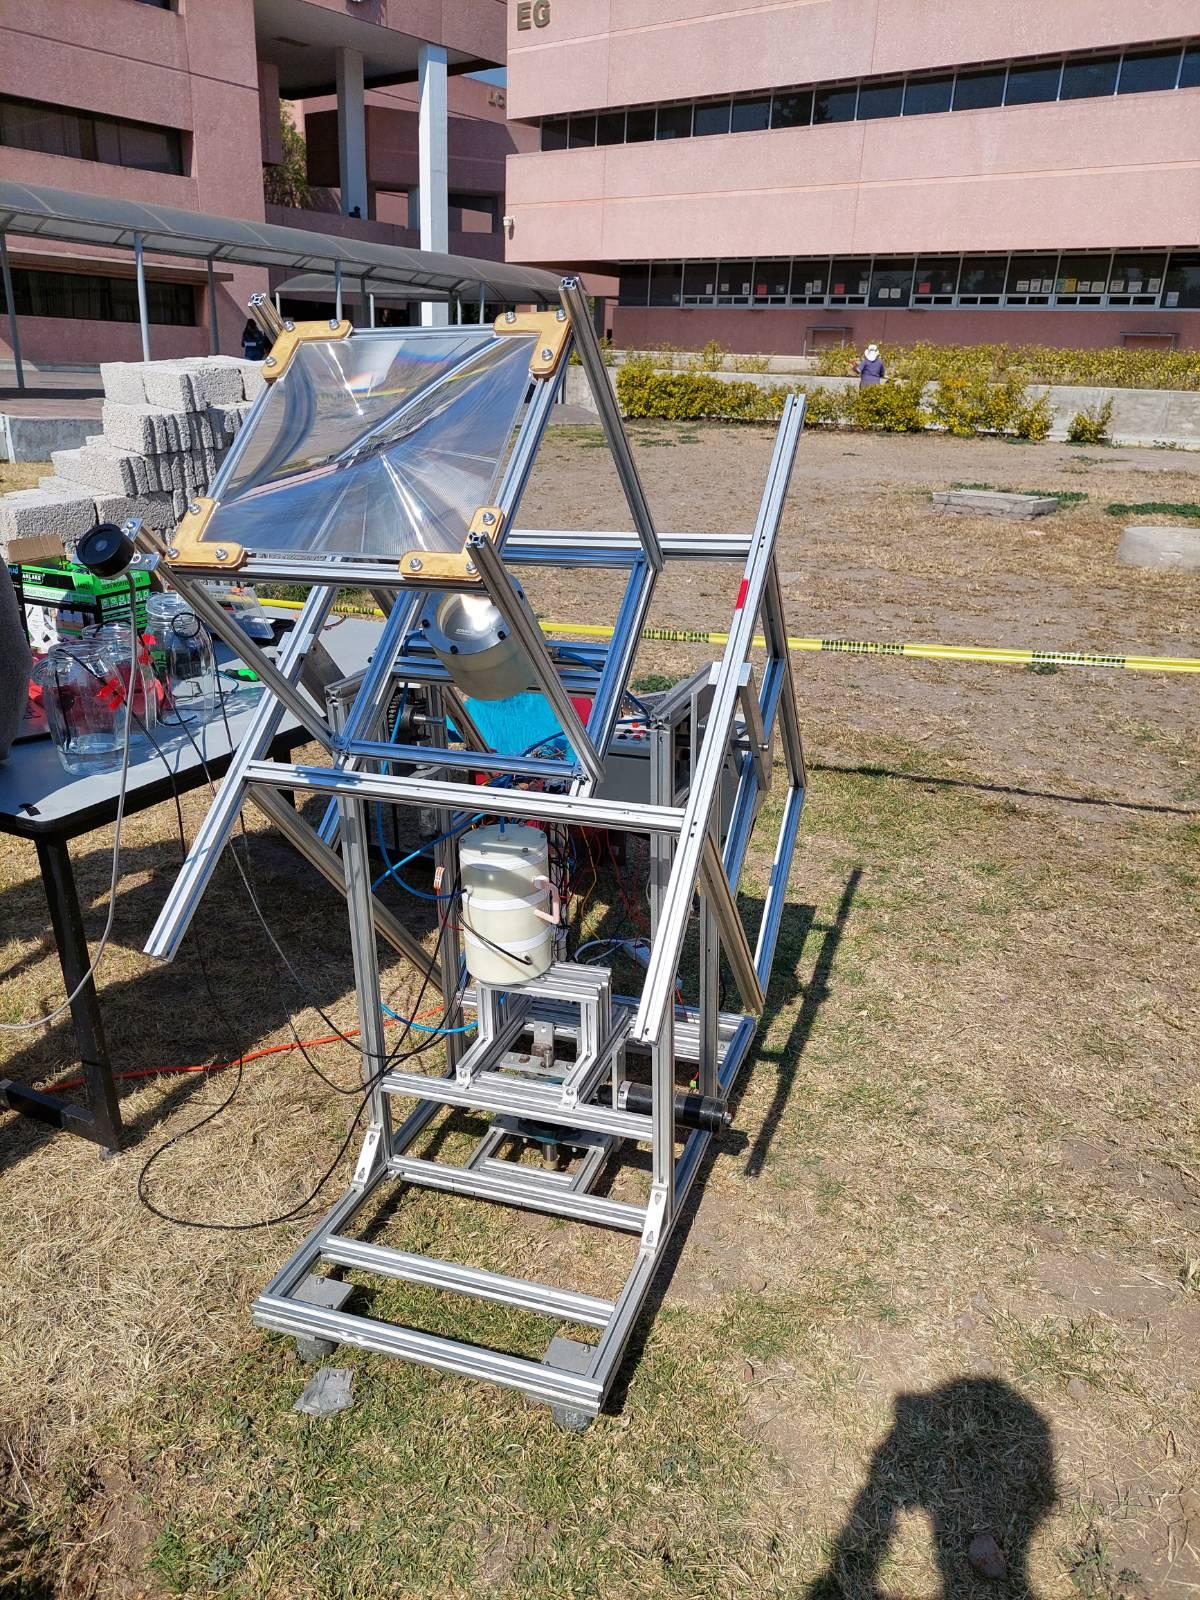
\includegraphics[
					height=70mm,
					width=\linewidth,
					keepaspectratio
				]{Resultados/Discusión/Ejecución.jpeg}
				\caption{Primer puesta en marcha del desalinizador}
			\end{figure}
		\end{column}
		\begin{column}{0.5\linewidth}
			\textbf{Hallazgos}
			
			\begin{itemize}
				\item Importancia del aislamiento térmico
				\item Implementación de estrategias de seguimiento solar
				\item Rediseños en el mecanismo de retroalimentación
				\item Excelente concentración: 3 min a \qty{860}{\watt\per\m\tothe{2}} para alcanzar temperatura de operación
			\end{itemize}
		\end{column}
	\end{columns}
\end{frame}

\begin{frame}
	\frametitle{Resultados}
	
	La evaluación del destilador solar se llevó acabo el día 16 de enero del 2024 entre las 13:30 y las 15:45 horas con un tiempo de funcionamiento de 2 horas
	
	\begin{columns}
		\begin{column}{0.5\linewidth}
			\vfill
			\begin{figure}
				\centering
				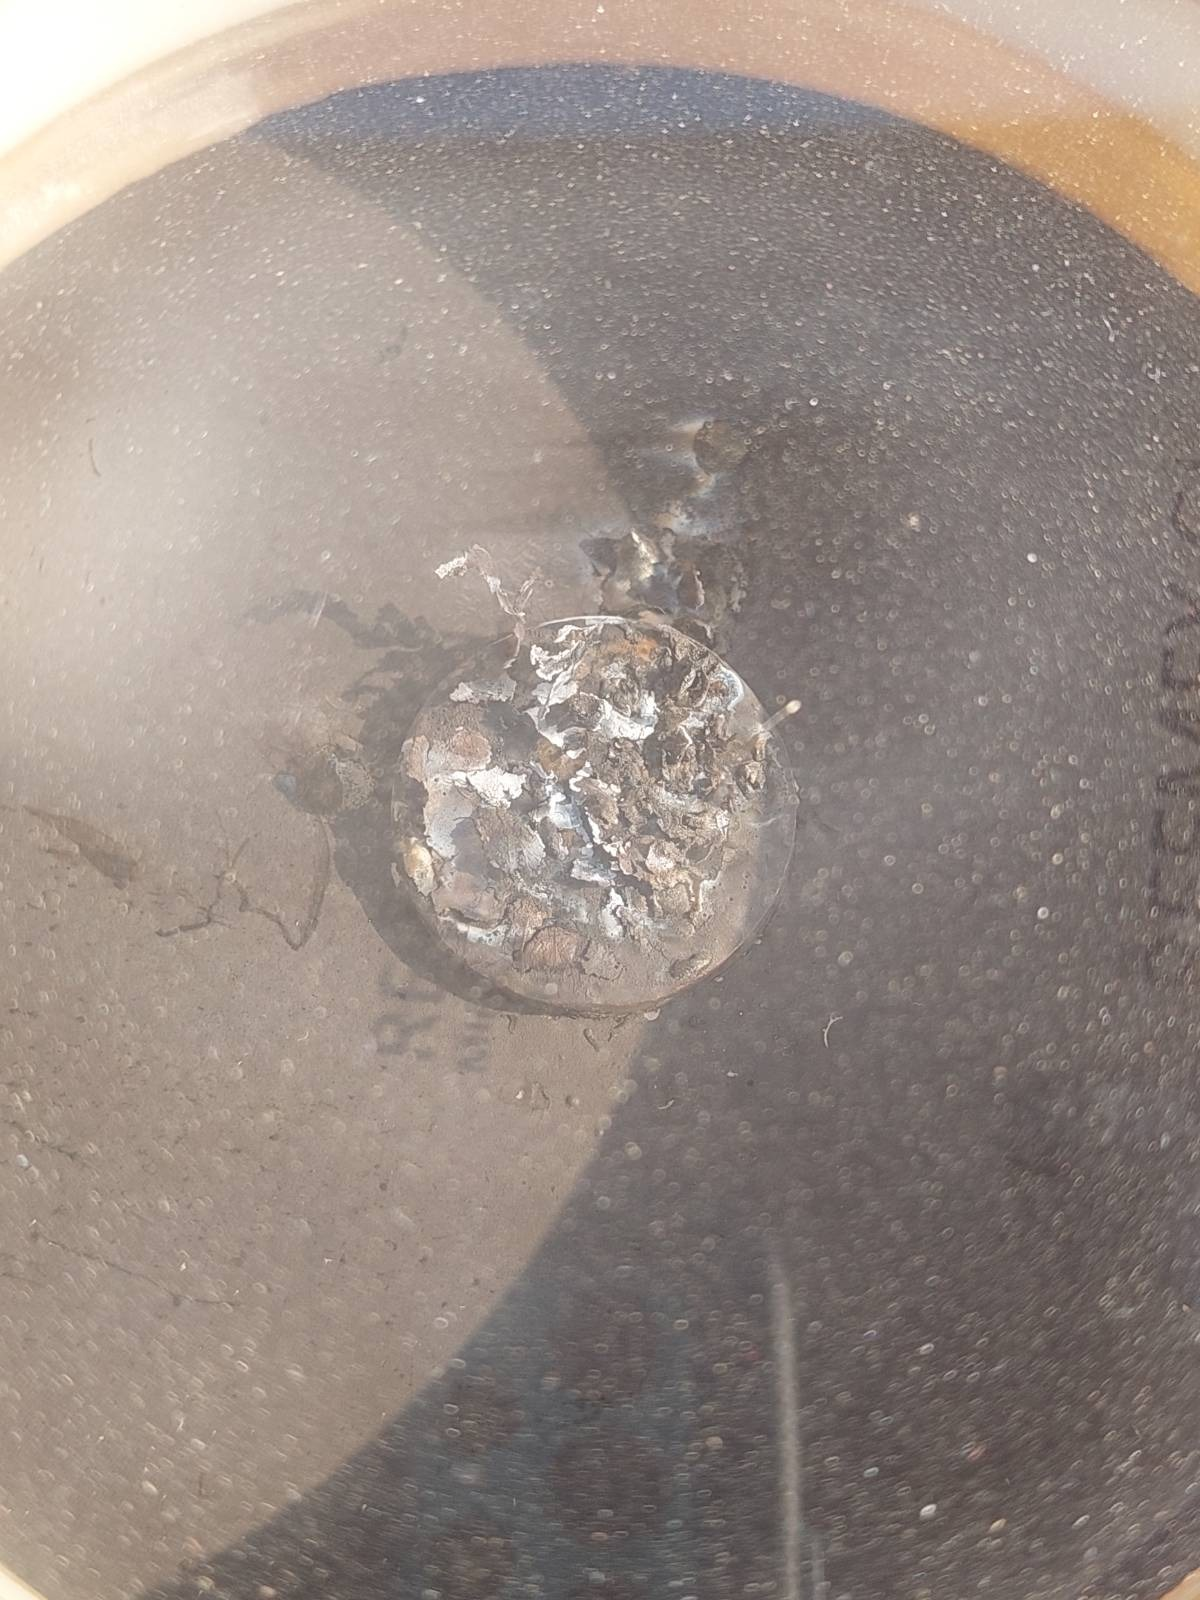
\includegraphics[
					height=50mm,
					width=\linewidth,
					keepaspectratio
				]{Resultados/Discusión/RecibidorQuemado.jpeg}
				\caption{Recibidor tras el primer uso}
			\end{figure}
		\end{column}
		\begin{column}{0.5\linewidth}
			\begin{figure}
				\centering
				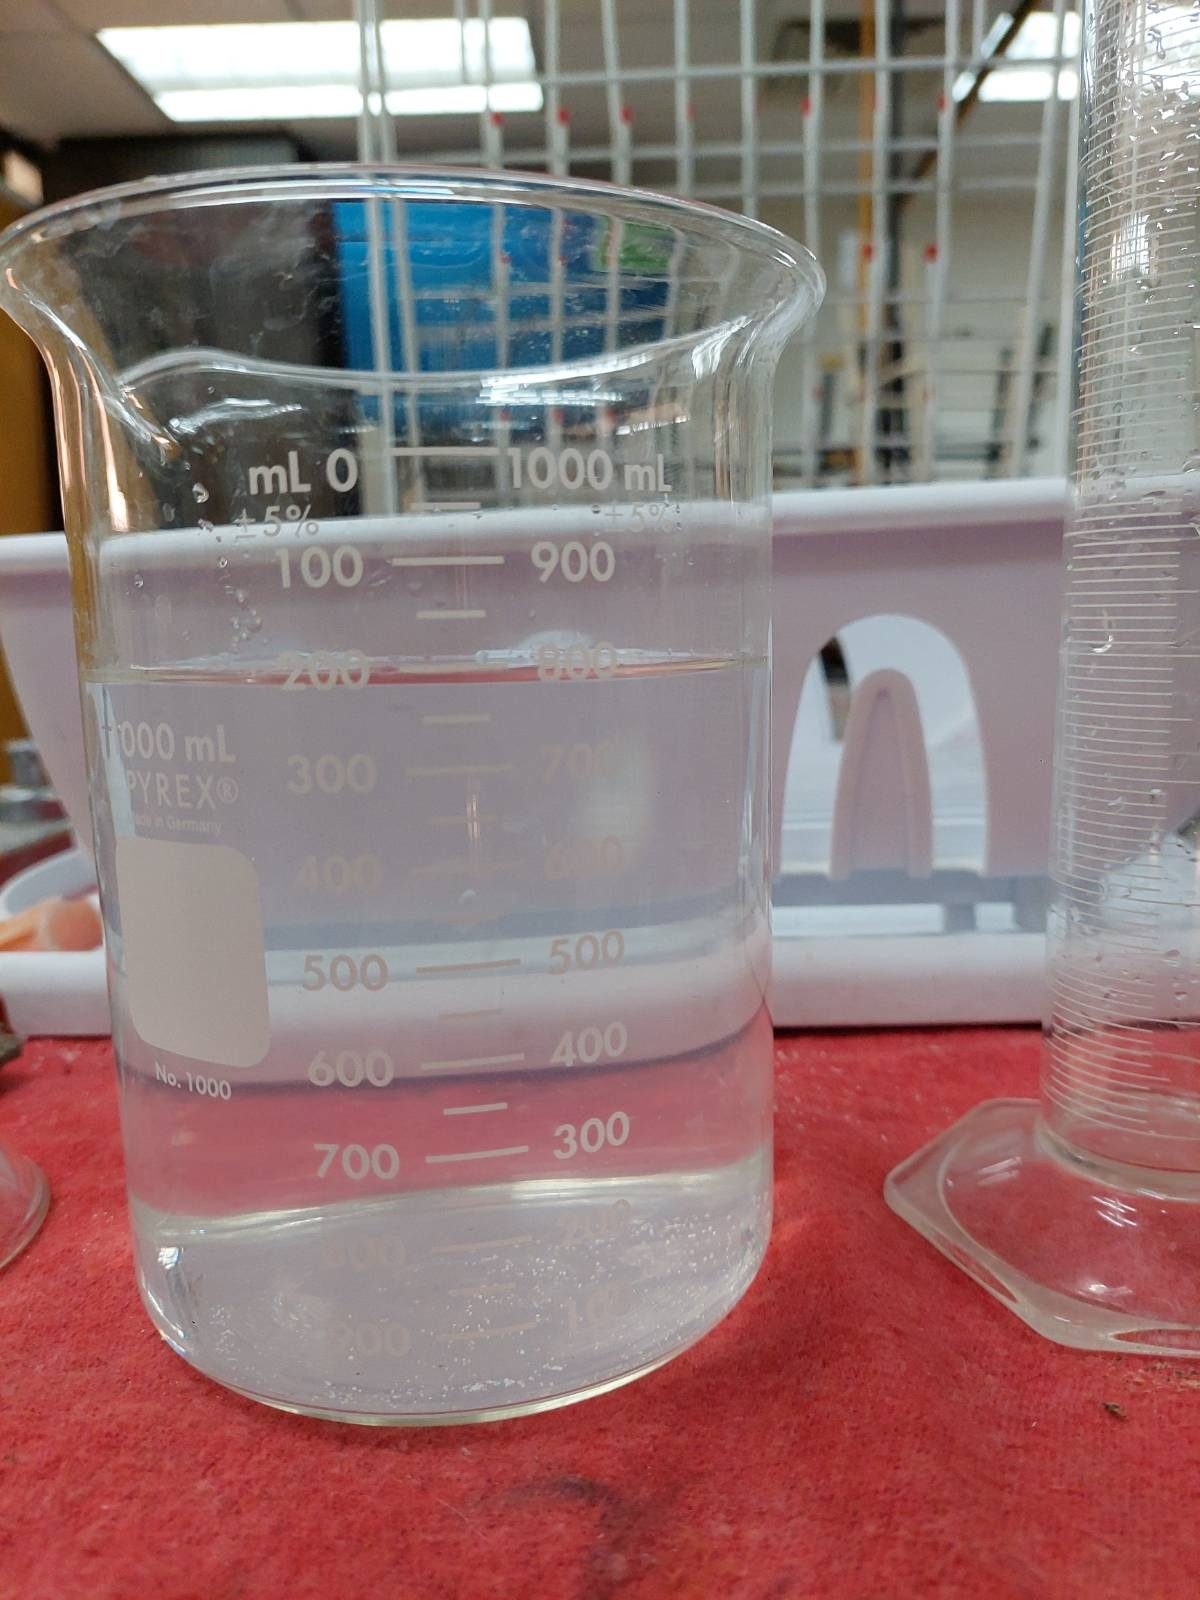
\includegraphics[
					height=50mm,
					width=\linewidth,
					keepaspectratio
				]{Resultados/Discusión/VasoPrecipitadosFinal.jpeg}
				\caption{Se lograron evaporar 194 mL de agua}
			\end{figure}
		\end{column}
	\end{columns}
\end{frame}

\begin{frame}
	\frametitle{Resumen}
	
	\begin{itemize}
		\item Se desarrollaron dos sistemas de control para el funcionamiento del desalinizador.
		\item Se consiguió completar todos los objetivos planteados.
		\item Durante la experimentación se identificaron las siguientes áreas de mejora en el diseño:
			\begin{itemize}
				\item Mecanismo de retroalimentación y condensación
				\item Concentración solar: seguimiento y recubrimientos
				\item Aislamiento térmico
			\end{itemize}
		\item Se destaca el valor teórico que aporta este trabajo al desarrollar una nueva propuesta que considera la separación física de los procesos de evaporación y condensación del agua así como la reutilización del calor generado.
	\end{itemize}	
	
\end{frame}